\documentclass[usenames,dvipsnames,tikz]{standalone}
\usepackage{xcolor}
\colorlet{myBlue}{RoyalBlue!35!Cerulean}
\colorlet{myRed}{Red!85!YellowOrange}
\usepackage{tikz}
\usepackage{standalone}
\begin{document}
	
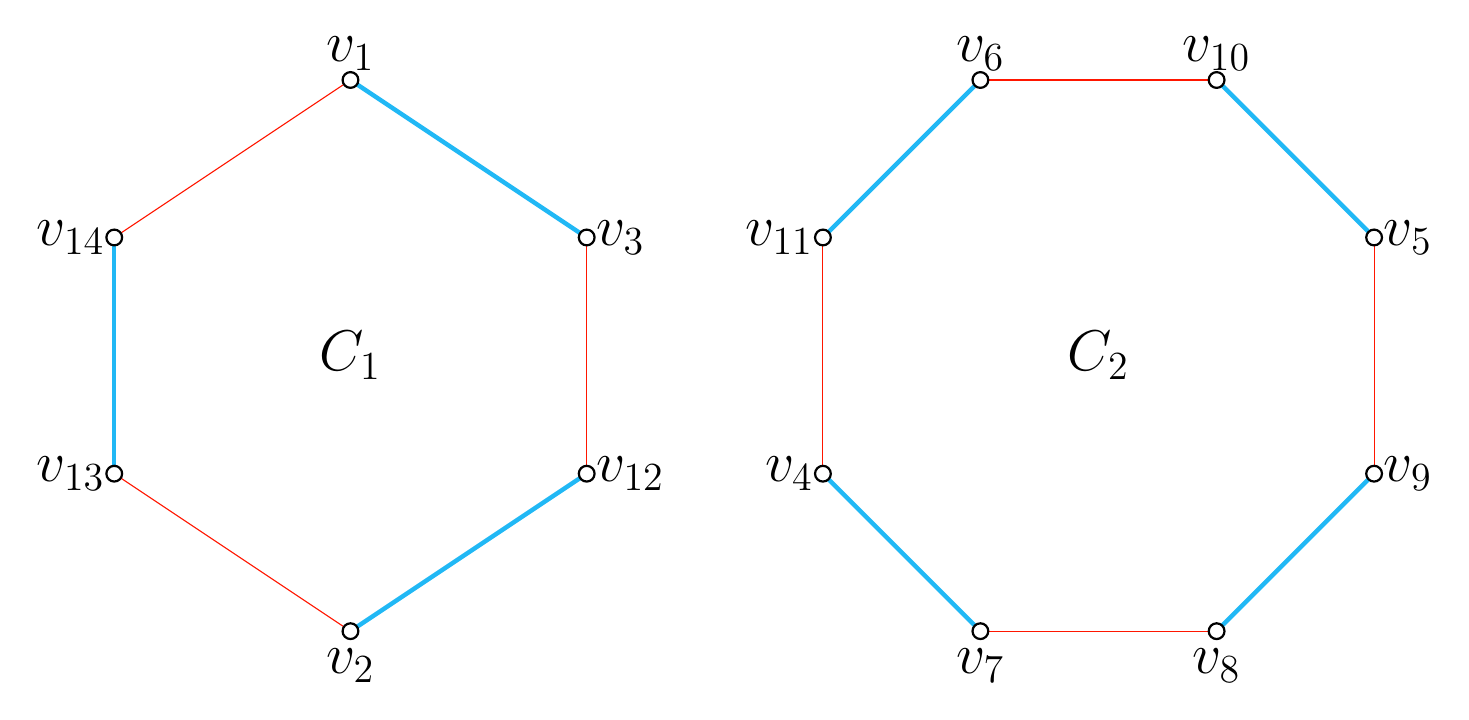
\begin{tikzpicture}
%\draw [help lines] (-1,-1) grid (25, 12);

%\draw [white] (4, -2.65) -- (12, -2.65);

\draw [ultra thick, myBlue] (4,0) -- (7,2);
\draw [ultra thick, myBlue] (4,7) -- (7,5);
\draw [ultra thick, myBlue] (1,2) -- (1,5);

\draw [ultra thick, myBlue] (10,2) -- (12,0);
\draw [ultra thick, myBlue] (15,0) -- (17,2);
\draw [ultra thick, myBlue] (15,7) -- (17,5);
\draw [ultra thick, myBlue] (12,7) -- (10,5);

\draw [myRed] (4,0) -- (1,2);
\draw [myRed] (4,7) -- (1,5);
\draw [myRed] (7,5) -- (7,2);

\draw [myRed] (10,2) -- (10,5);
\draw [myRed] (12,7) -- (15,7);
\draw [myRed] (17,5) -- (17,2);
\draw [myRed] (15,0) -- (12,0);

\draw [fill=white, thick] (4,0) circle [radius = 0.1];
\draw [fill=white, thick] (1,2) circle [radius = 0.1];
\draw [fill=white, thick] (7,2) circle [radius = 0.1];
\draw [fill=white, thick] (1,5) circle [radius = 0.1];
\draw [fill=white, thick] (7,5) circle [radius = 0.1];
\draw [fill=white, thick] (4,7) circle [radius = 0.1];

\draw [fill=white, thick] (10,2) circle [radius = 0.1];
\draw [fill=white, thick] (10,5) circle [radius = 0.1];
\draw [fill=white, thick] (17,2) circle [radius = 0.1];
\draw [fill=white, thick] (17,5) circle [radius = 0.1];
\draw [fill=white, thick] (12,0) circle [radius = 0.1];
\draw [fill=white, thick] (12,7) circle [radius = 0.1];
\draw [fill=white, thick] (15,0) circle [radius = 0.1];
\draw [fill=white, thick] (15,7) circle [radius = 0.1];


\node [below] at (4,-0.1) {\huge{$v_2$}};
\node [left] at (1,2) {\huge{$v_{13}$}};
\node [left] at (1,5) {\huge{$v_{14}$}};
\node [above] at (4,7) {\huge{$v_1$}};
\node [right] at (7,5) {\huge{$v_3$}};
\node [right] at (7,2) {\huge{$v_{12}$}};

\node [below] at (15,-0.1) {\huge{$v_8$}};
\node [below] at (12,-0.1) {\huge{$v_7$}};
\node [left] at (10,2) {\huge{$v_4$}};
\node [left] at (10,5) {\huge{$v_{11}$}};
\node [above] at (12,7) {\huge{$v_6$}};
\node [above] at (15,7) {\huge{$v_{10}$}};
\node [right] at (17,5) {\huge{$v_5$}};
\node [right] at (17,2) {\huge{$v_9$}};

\node at (4,3.5) {\huge{$C_1$}};
\node at (13.5, 3.5) {\huge{$C_2$}};








\end{tikzpicture}
	
\end{document}
